\documentclass[../../../../main.tex]{subfiles}

\begin{document}

\subsection{Hough Transform - Implementation}
\label{sec:cv_hough_impl}
As a way of implementing the Hough transform the OpenCV function
is used.\\

\texttt{ HoughCircles(src\_gray,circles\_list,CIRC\_DETECT\_METHOD,inv\_resol\_ratio,u\_Canny\_det) }\\

By observing the camera image, a large proportion of noise can be seen. To reduce the effect of this, a Gaussian filter with a mask size of 5 is applied with
\texttt{GaussianBlur()}.
The image from the camera is then converted to grayscale and used in
\texttt{HoughCircles()}. \\

\begin{figure}[h]
  \begin{center}
	\subfloat[Marble detection with colors.]{%
		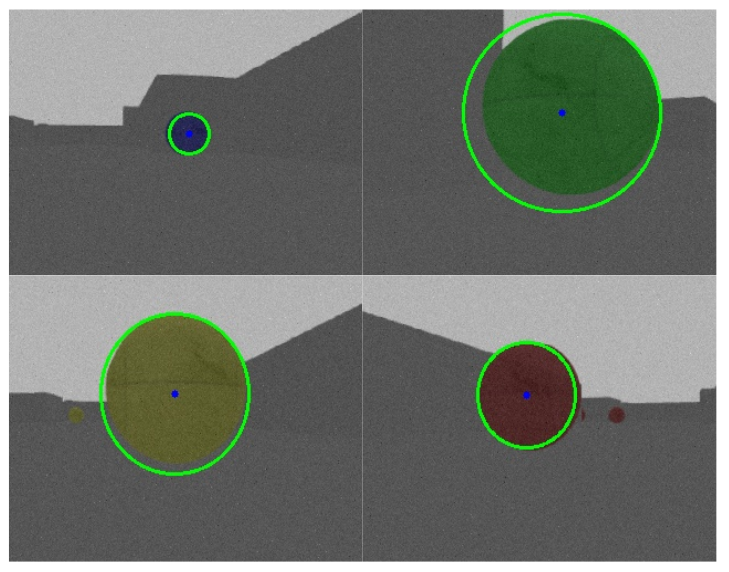
\includegraphics[width=0.49\textwidth]{%
		\main/afsnit/cv/methods/hough_circ/cv_hough_detect_colors.png}
	}
	\subfloat[Marble detection without colors.]{%
    \includegraphics[width=0.505\textwidth]{%
		\main/afsnit/cv/methods/hough_circ/cv_hough_shapes.png}
	}
  \end{center}
	\caption{Marble detection with and without colors.}
	\label{fig:hough_colors}
\end{figure}

For appropriate use this method's, default inputs are used for the circle list, detection method, inverse ratio of solution, Canny detection's upper threshold, minimum radius and maximum radius.\\

Therefore the tuned values are the minimal distance between circles and the threshold for center detection.\\

When determining threshold for center detection, it is important to consider the instability of the Hough transform. Therefore the value of center detection is tuned to reduce this instability, resulting in a more robust evaluation of contrast in the image, when detecting marble edges.\\

%\begin{wrapfigure}{r}{0.4\textwidth}
%	\vspace{-1cm}
%  \begin{center}
%    \includegraphics[width=0.38\textwidth]{\main/afsnit/cv/methods/hough_circ/cv_hough_shapes.png}
%  \end{center}
%  \caption{Marble detection without colors.}
%  \label{fig:hough_shapes}
%\end{wrapfigure}

The tuning has greatly reduced the number of false positive circles detected. When testing the performance of this tuning, another challenge surfaces.
There are two challenges, one being that when there is a very small distance between the marbles, the Hough transform seems to flicker between the marbles, thus causing the agent to move in a sinusoidal pattern. The other variation is when the agent are close enough to a marble that it takes up most of the scene, the instability of the Hough transform becomes more influential and a large number of widespread Hough circles are detected. To solve both of these problems, the parameter determining the distance between marbles we wish to detect is tuned.\\
Now having tuned these parameters, the results can be seen applied on different colors on figure \ref{fig:hough_colors}.
\end{document}
